% ---------------------------------------------------------------------------
% Problem Set 3: Replication Report Empirical Methods
% The grey instructions are produced by \instr{...}. To hide all of them at once (e.g. to check the length of your report), change \showinstrtrue to \showinstrfalse below. Please remove them before you submit.
% ---------------------------------------------------------------------------
\documentclass[12pt,a4paper]{article}

\usepackage[utf8]{inputenc}
\usepackage[T1]{fontenc}
\usepackage{mathptmx}
\usepackage{microtype}
\usepackage[margin=2.5cm]{geometry}
\usepackage{amsmath,amssymb}
\usepackage{graphicx}
\usepackage{float}
\usepackage{booktabs}
\usepackage{tabularx}
\usepackage{array}
\usepackage{colortbl}
\usepackage{enumitem}
\usepackage{xcolor}
\usepackage[font=small,labelfont=bf,skip=6pt]{caption}
\usepackage[hidelinks]{hyperref}
\usepackage{titlesec}
\titleformat*{\section}{\large\bfseries}
\titleformat*{\subsection}{\normalsize\bfseries}
\titlespacing*{\section}{0pt}{12pt}{6pt}
\titlespacing*{\subsection}{0pt}{8pt}{4pt}

\setlength{\parindent}{0pt}
\setlength{\parskip}{6pt}
\usepackage{tabularx}
\usepackage{array}
\usepackage{booktabs}
\newcolumntype{L}{>{\raggedright\arraybackslash}X}

% --- Instructions ----------------------------------------------------------
\newif\ifshowinstr
%\showinstrtrue
\showinstrfalse
\newcommand{\instr}[1]{\ifshowinstr{\leavevmode\color{gray}\itshape\small [#1]\par}\fi}

% --- Helpers for the worksheets --------------------------------------------
\newcolumntype{L}{>{\raggedright\arraybackslash}X}
\newcolumntype{P}[1]{>{\raggedright\arraybackslash}p{#1}}
\newcommand{\fillrow}{\rule[-0.35cm]{0pt}{0.85cm}}  % leaves room to write in a row
\newcommand{\rowline}{\arrayrulecolor{black!25}\hline\arrayrulecolor{black}}
\renewcommand{\arraystretch}{1.25}

% --- Table notes -----------------------------------------------------------
\newcommand{\tablenotes}[1]{\par\vspace{4pt}{\footnotesize\textit{Notes:} #1\par}}

\title{Replication of Alesina, Giuliano \& Nunn (2013):\\{} On the Origins of Gender Roles: Women and the Plough}
\author{\begin{tabular}{c@{\hspace{2.5em}}c}Ginevra Bettata & Isimbi Elsa Usanase\\ Leandra Shana Grossniklaus & Rahel Tiffany Gutzwiller\end{tabular}}

\predisplaypenalty=0
\begin{document}
\maketitle

\instr{The grey italic passages provide you with some short instructions. Please delete these passages before you submit by setting \texttt{\textbackslash showinstrfalse} in the preamble. \textbf{The report should be 5 to 7 pages long.} This includes tables and figures but excludes any references and Appendix A. \textbf{Appendix A} tries to guide you through some of the replication exercises. It \textbf{has to be filled in and submitted together with the report}. Appendix~B is only meant as a help for you, and you can delete it before submitting.}

% ===========================================================================
\section{Introduction}
% ===========================================================================
% Problem and research question
Gender norms differ strongly across countries, even at similar income levels: in 2000, female labour force participation was 16.1\% in Pakistan but 90.5\% in Burundi. Alesina, Giuliano and Nunn (2013) test whether these differences go back to traditional plough agriculture, as Ester Boserup (1970) argued. Because the plough requires upper-body strength and is difficult to combine with childcare, men worked in the fields while women worked at home, and this division of labour turned into a lasting belief about women's role.

% Method and findings
The authors link ethnographic data on ancestral plough use to today's countries and estimate OLS regressions with historical and contemporary controls, as well as 2SLS regressions that instrument plough use with the suitability of ancestral land for crops that benefit more or less from the plough. A country whose population descends entirely from plough-using societies has 12.9 percentage points lower female labour force participation than a country with no plough tradition (Table IV, column 2, of the paper); under 2SLS, the difference rises to 25.0 percentage points.

% Our contribution
We replicate these OLS and IV results exactly. In our extension, we ask whether communist regimes, which actively pushed women into paid work, weakened the plough effect. We find no evidence of this: the implied effect is about $-11$ percentage points in (former) communist countries and $-14.5$ elsewhere, and the difference is not significant. Our critical evaluation argues that the main biases in the OLS estimate pull in opposite directions and that the exclusion restriction of the IV is questionable, so the sign of the effect is more credible than its size.

% ===========================================================================
\section{Data and Methodology}
% ===========================================================================
\instr{Think about what you need to explain the identification strategy of the authors and why they believe that it is valid. Appendix~B.1 summarizes the main points for OLS, panel data and IV designs. You can use these as a reference.}

The main result comes from a cross-country regression:
\begin{equation}\label{eq:ols}
  FLFP_c = \alpha + \beta\, Plough_c + (X_c^{H})'\gamma + (X_c^{C})'\delta + \mu_{continent} + \varepsilon_c
\end{equation}
$FLFP_c$ is the female labour force participation rate in 2000, expressed as a percentage. $Plough_c$ is the share of the population whose ancestors used the plough, ranging from zero to 1. $X_c^{H}$ contains historical controls describing the ancestors: the agricultural suitability of the land, the tropical climate, the presence of large domesticated animals and the political and economic complexity of the ancestors. The contemporary controls $X_c^{C}$ are the logarithm of real per capita GDP and its square. The term $\mu_{continent}$ captures continent fixed effects.

The authors acknowledge that, $\beta$ measures a causal effect only if one assumes that, holding controls constant, plough is not correlated with anything else that might influence female labour force participation. The authors add a range of other controls (Table VII), but these cannot account for what is not observed.

To identify this effect, the authors turn to two-stage least squares (2SLS). The idea comes from Pryor (1985) who argued that the plough is particularly advantageous for crops that require a large amount of land to be prepared in a short time, on deep and flat soils. The first measure is the suitability of ancestral lands for wheat, barley and rye, for which the plough is highly advantageous (plough-positive environment). The second is the suitability for sorghum and millet, for which the use of the plough was less advantageous (plough-negative environment). We express the first-stage specification described by Alesina, Giuliano and Nunn (2013, p.~516) as follows:
\begin{equation}\label{eq:firststage}
  Plough_c = \pi_0 + \pi_1\, PosEnv_c + \pi_2\, NegEnv_c + X_c'\lambda + \mu_{continent} + u_c
\end{equation}
In the second stage they substitute $Plough_c$ with the value predicted in the first stage in the original regression equation.

The method is based on four assumptions. The first is relevance, whereby, holding controls constant, the instruments must explain plough use. The second is exogeneity: the instruments must not be correlated with unobserved factors. The authors argue that this is plausible because climate and soil are determined by nature. The third assumption is the exclusion restriction: the types of cereal crops that can be grown must affect current female labour force participation only through plough use. The authors themselves acknowledge that this cannot be taken for granted. The fourth is monotonicity, which is necessary when effects differ across societies and the 2SLS estimates a local effect (LATE). Under this assumption, greater suitability for wheat must never make a society less likely to adopt the plough.

The first threat to this strategy is weak instruments, if the instruments only weakly predict plough use (weak first stage), the 2SLS model approaches OLS and standard tests are unreliable.

The second threat is that the exclusion may not hold. Geography may have shaped development, population density, the emergence of states or nutrition, which in turn may have influenced gender norms. In Table A14, they also control for slope, soil depth, temperature and precipitation, but other channels remain possible.

% ===========================================================================
\section{Main Result}
% ===========================================================================

\subsection{OLS results}

\instr{This part should include your main replication table (Table~\ref{tab:main}) and figure(s) (at least Figure~\ref{fig:main}). Replicate at least what you consider the main column of the main results table, as well as one or two figures that visualize the result. Do your results differ? Worksheet~A.3 helps you think about why they might differ. It is fine if you cannot replicate a number exactly, as long as you understand why.}

We first replicate the authors' OLS estimates of the relationship between traditional plough use and female labour force participation in 2000. Because plough use is measured as the share of each country's population with plough-using ancestors, the analysis is a cross-country regression with one observation per country. Our main specification estimates equation~\eqref{eq:ols} on 165 countries. Besides plough use, it includes the historical controls, which describe how the ancestors lived, and income, which captures today's level of development. The continent fixed effects mean that each country is only compared with countries on the same continent, so broad regional differences, for example between Africa and Europe, cannot drive the result. As in the paper, standard errors are robust to heteroskedasticity. Table~\ref{tab:main} presents the estimated regressions side by side. Columns (1) and (2) replicate Table III in the paper, which does not yet include income as a contemporary control. Columns (3) and (4) replicate Table IV in the paper, which adds income. Columns (2) and (4) include continent fixed effects, and column (4), which corresponds to Table IV, column (2) in the paper, is our main specification.

\begin{table}[H]
  \centering
  \vspace{-4pt}
  \caption{Country-level OLS estimates of female labour force participation in 2000 (replication of Tables III and IV)}
  \label{tab:main}
  \small
  \renewcommand{\arraystretch}{1}
  \setlength{\tabcolsep}{11.5pt}
  
\begin{tabular}[t]{lcccc}
\toprule
\multicolumn{1}{c}{ } & \multicolumn{2}{c}{Table III} & \multicolumn{2}{c}{Table IV} \\
\cmidrule(l{3pt}r{3pt}){2-3} \cmidrule(l{3pt}r{3pt}){4-5}
\multicolumn{1}{c}{\em{ }} & \multicolumn{4}{c}{\em{Dependent variable: female labour force participation in 2000}} \\
\cmidrule(l{3pt}r{3pt}){2-5}
 & (1) & (2) & (3) & (4)\\
\midrule
Traditional plough use & -14.895*** & -15.962*** & -12.401*** & -12.930***\\
 & (3.318) & (3.881) & (2.964) & (3.537)\\
\addlinespace[0.3em]
\multicolumn{5}{l}{\textit{Historical controls:}}\\
\hspace{1em}Agricultural suitability & 9.407** & 9.017** & 6.073 & 7.181*\\
\hspace{1em} & (3.885) & (4.236) & (3.696) & (4.175)\\
\hspace{1em}Tropical climate & -8.644*** & -12.389*** & -9.718*** & -10.906***\\
\hspace{1em} & (2.698) & (3.302) & (2.487) & (3.070)\\
\hspace{1em}Presence of large animals & 10.903** & 2.350 & -2.015 & -2.166\\
\hspace{1em} & (5.032) & (5.956) & (5.372) & (6.072)\\
\hspace{1em}Political hierarchies & -0.787 & 0.447 & 0.779 & 1.181\\
\hspace{1em} & (1.622) & (1.624) & (1.515) & (1.482)\\
\hspace{1em}Economic complexity & 0.170 & 1.157 & 1.157 & 1.411*\\
\hspace{1em} & (0.849) & (0.859) & (0.793) & (0.815)\\
\addlinespace[0.3em]
\multicolumn{5}{l}{\textit{Contemporary controls:}}\\
\hspace{1em}ln income in 2000 &  &  & -34.612*** & -32.685***\\
\hspace{1em} &  &  & (6.528) & (7.023)\\
\hspace{1em}ln income in 2000 squared &  &  & 2.038*** & 1.936***\\
\hspace{1em} &  &  & (0.406) & (0.431)\\
\midrule
Continent fixed effects & no & yes & no & yes\\
Observations & 177 & 177 & 165 & 165\\
Adjusted R-squared & 0.19 & 0.24 & 0.37 & 0.36\\
R-squared & 0.22 & 0.28 & 0.40 & 0.41\\
Mean of dep. var. & 51.03 & 51.03 & 51.35 & 51.35\\
\bottomrule
\multicolumn{5}{l}{\rule{0pt}{1em}*** p < 0.01, ** p < 0.05, * p < 0.1.}\\
\end{tabular}

\end{table}

We obtain the same coefficients and standard errors as the authors, up to the third decimal, since we use the data used by the authors and the same specification. The only exception is the adjusted R-squared in column (1), where we obtain 0.19 instead of 0.20, a rounding difference. In our main specification, the coefficient on traditional plough use is $-12.93$ (SE 3.54). Going from a country where no ancestors used the plough to one where all did is associated, on average, with a 12.93 percentage points lower female labour force participation rate, holding the controls and the continent constant. A one-standard-deviation increase in plough use (0.47) is associated with a 6.10 percentage points lower rate, which is about 12\% of the average participation rate of 51.35\%. The coefficient is statistically significant at the 1\% level ($t = -3.66$; 95\% confidence interval from $-19.92$ to $-5.94$) and economically large. The estimate is also stable, as it lies between $-12.4$ and $-16.0$ in all four columns. With respect to our research question, the results show that countries with a plough tradition have markedly lower female labour force participation today. So far, however, this is a correlation and not yet proof of a causal effect.

Figure~\ref{fig:main} shows this relationship graphically. A simple scatter plot of participation against plough use would also reflect differences in the controls, for example that plough countries differ in income and climate. To show only the relationship that the regression measures, we first remove from both variables the part that the controls can explain and then plot the remaining residuals against each other. By the Frisch--Waugh--Lovell theorem, the slope of the fitted line equals the OLS coefficient. The figure replicates Figure IVa of the paper, which is based on Table IV, column (1) in the paper and has no continent fixed effects. It reproduces the published figure with the same slope of $-12.40$. The negative relationship is visible across many countries.

\begin{figure}[H]
  \centering
  \caption{Partial regression plot of female labour force participation in 2000 on traditional plough use (replication of Figure IVa)}
  \label{fig:main}
  \vspace{6pt}
  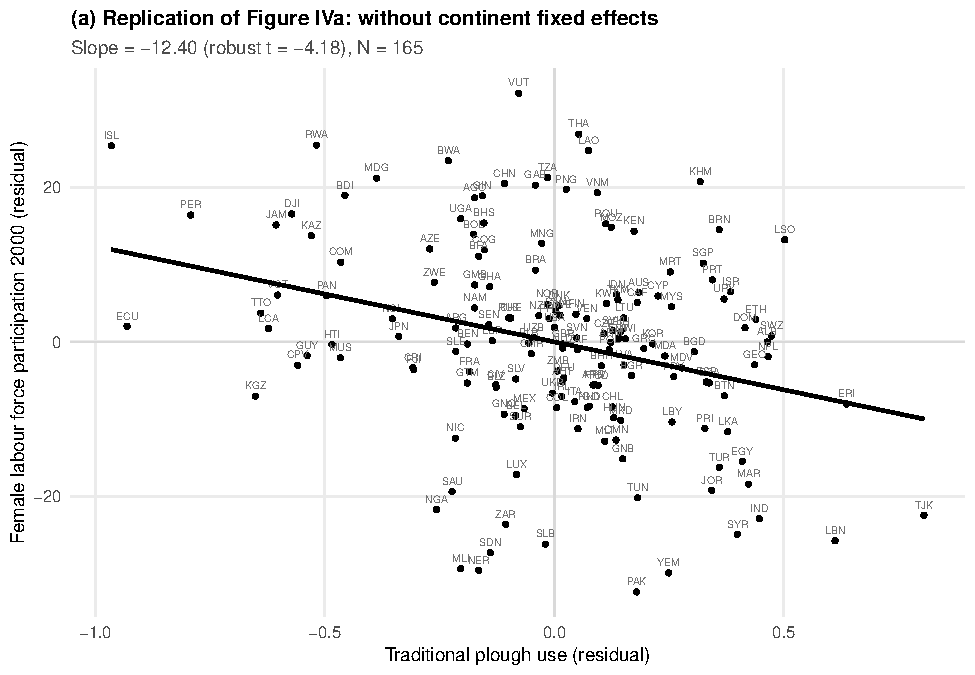
\includegraphics[width=\textwidth]{figures/figure_iva_replication.pdf}
\end{figure}

We learn that plough ancestry is strongly associated with lower female labour force participation today, and our replication confirms the authors' numbers. Whether this association reflects a causal effect is examined with the IV estimates in Section~\ref{sec:iv}.

\subsection{IV results}\label{sec:iv}

\begin{table}[H]
  \centering
  \vspace{-4pt}
  \caption{IV replication of Alesina et al.\ (2013), Table VIII, column (2)}
  \label{tab:iv_replication}
  \small
  \renewcommand{\arraystretch}{1}
  \setlength{\tabcolsep}{11.5pt}
  
\begin{tabular}{llrrr}
\toprule
Model & Regressor & Estimate & Robust SE & p-value\\
\midrule
First stage & Plough-positive crop suitability & 0.629 & 0.089 & < 0.001\\
 & Plough-negative crop suitability & 0.185 & 0.133 & 0.16563\\
Reduced form & Plough-positive crop suitability & -11.299 & 4.285 & 0.00928\\
 & Plough-negative crop suitability & 19.571 & 6.329 & 0.00238\\
2SLS & Traditional plough use & -25.013 & 7.513 & 0.00110\\
\addlinespace
Same-sample OLS & Traditional plough use & -12.089 & 3.587 & < 0.001\\
\bottomrule
\end{tabular}


  \tablenotes{All models use the same 160 countries and include historical controls, contemporary income controls and continent fixed effects. The first-stage outcome is traditional plough use. The outcome in the other models is female labour force participation in 2000.}
\end{table}

Table~\ref{tab:iv_replication} shows that suitability for plough-positive crops is the stronger first-stage predictor of traditional plough use and the joint first-stage $F$-statistic of 25.06 supports instrument
relevance.
In the reduced form, the two crop-suitability measures are associated with female labour force participation in opposite directions.
A 10-percentage-point increase in traditional plough use corresponds to about 2.5 percentage points lower female labour force participation in the 2SLS model, compared with 1.2 percentage points in OLS on the same
sample.
The Hansen $J$ test rejects the overidentifying restrictions, which calls for caution when interpreting the 2SLS estimate as causal or relying on the Hausman test, whose interpretation assumes valid instruments.

% ===========================================================================
\section{Critical Evaluation}
% ===========================================================================
\subsection{Threats to internal validity}

For $\beta$ to measure a causal effect, plough use must be uncorrelated with the error term, conditional on the controls: $E[\varepsilon_c \mid Plough_c, \mathbf{X}_c] = 0$. We discuss three reasons why this may fail and then ask whether the IV strategy solves them.

\paragraph{Threat 1: Pre-existing gender norms (OVB and reverse causality).}

As the authors themselves acknowledge, male-dominated societies may have been more likely to adopt the plough, so causality could also run from norms to plough use. If these norms were passed down, they also lower FLFP today and are part of the error term. Using the OVB formula from class,
\[
E(\hat\beta) = \beta + \gamma_z \, \hat\beta_{z\_on\_plough} ,
\]
where $z$ stands for pre-existing norms, $\gamma_z$ for their effect on FLFP and $\hat\beta_{z\_on\_plough}$ for the coefficient on plough use in a regression of $z$ on plough use and the controls. Plough use is positively related to unequal norms ($\hat\beta_{z\_on\_plough} > 0$), and unequal norms reduce FLFP ($\gamma_z < 0$). The bias is therefore negative and moves the estimate away from zero, so OLS overstates the effect of the plough. Religion, one channel through which such norms are transmitted, gives a sense of the size: controlling for it reduces the coefficient from $-12.4$ to $-9.9$, about 20\% (Table VII, without continent fixed effects). Since religion is measured in 2000, it captures norms from before the plough only partly, so the true bias may be larger.

\paragraph{Threat 2: Development and income.}

Societies that adopted the plough were more developed, and their descendants are richer today. Unlike pre-existing norms, income is observed and included as a control, which lets us measure how large such a bias can be. When we drop log income and its square from our main specification, the coefficient moves from $-12.93$ to $-16.47$. Since two variables are omitted, the bias has two terms:
\[
\text{bias} = \delta_1 \, \hat\beta_{inc\_on\_plough} + \delta_2 \, \hat\beta_{inc^2\_on\_plough} = -33.98 + 30.44 = -3.54 ,
\]
where $\delta_1 = -32.69$ and $\delta_2 = 1.94$ are the coefficients on log income and its square in equation~\eqref{eq:ols}, and $\hat\beta_{inc\_on\_plough} = 1.04$ and $\hat\beta_{inc^2\_on\_plough} = 15.72$ are the coefficients on plough use in regressions of log income and its square on plough use and the other controls. The formula reproduces the gap exactly, and the bias moves the estimate away from zero. The net sign is negative because of the U-shaped relationship between income and female participation, which is also why the authors include the square of log income (Goldin, 1995). 72\% of our countries lie below the turning point of the estimated U-curve, $\exp(-\delta_1 / 2\delta_2) \approx$ USD 4,600, where higher income goes along with fewer working women, and plough countries are richer on average. If income is partly a consequence of the plough, it is a bad control and part of the $-3.54$ belongs to the plough effect. The total effect would then lie between $-12.9$ and $-16.5$.

\paragraph{Threat 3: Measurement error.}

Each ethnic group is only coded as having used the plough or not, and these groups are then linked to today's countries through ancestry, so plough use is measured with error. Classical measurement error pulls the coefficient towards zero (attenuation bias), so OLS understates the effect. This works in the opposite direction to Threat 1.

\paragraph{Does the IV strategy solve these problems?}

The instruments are the suitability of ancestral land for crops that benefit strongly from the plough (wheat, barley, rye) and for crops that benefit little (sorghum, millet). Since gender norms cannot change soil or climate, the instruments can address the reverse causality in Threat 1, and 2SLS also corrects for classical measurement error. The 2SLS estimate ($-25.0$) is about twice as large in absolute value as OLS on the same 160 countries ($-12.1$), and, if the instruments are valid, the Hausman test rejects the exogeneity of plough use ($p = 0.04$). This contradicts Threat 1, which predicts that OLS is too negative, but is consistent with measurement error dominating.

However, the IV is only valid if crop suitability affects FLFP solely through plough use, i.e.\ $\operatorname{Cov}(Z, \varepsilon) = 0$. Because crop suitability reflects geography, regions suited to plough-positive and plough-negative crops may also differ in disease burden, economic development or the type of farm work the crops require. The authors control for overall agricultural suitability and tropical climate, but other differences may remain in the error term, and the data support this concern. The Hansen J test rejects ($J = 14.9$, $p < 0.001$), and suitability for plough-negative crops barely predicts plough use (first stage: $0.18$, $p = 0.17$) but strongly predicts FLFP (reduced form: $19.6$, $p = 0.002$). This points to a direct effect that does not run through the plough. Since Hansen J only tests whether the two instruments agree, it could not detect a case where both are invalid in the same way. Table~\ref{tab:threats} summarises the threats.

\begin{table}[H]
\centering
\caption{Threats to internal validity and their likely effect on the OLS estimate}
\label{tab:threats}
\small
\begin{tabular}{llll}
\hline
Threat & Direction of bias & Effect on $-12.9$ & Solved by IV? \\
\hline
Pre-existing norms & negative & overstated & only if exclusion restriction holds \\
Development and income & negative ($-3.5$) & controlled for & observed; possibly a bad control \\
Measurement error & towards zero & understated & yes, if error is classical \\
IV: exclusion restriction & unclear & -- & doubtful (Hansen J rejects) \\
\hline
\end{tabular}
\end{table}

\subsection{Overall assessment}

We find the paper's main claim convincing in direction but not in magnitude. The main threats bias the OLS estimate in opposite directions, and the IV strategy rests on a questionable exclusion restriction, so we cannot say whether $-12.9$ over- or understates the true effect. Still, the negative relationship holds across several outcomes, many additional controls (Table VII) and our own extension, and the evidence on children of immigrants, who live under the same institutions, makes a purely geographic or institutional explanation unlikely. We therefore consider it credible that traditional plough use contributed to today's gender norms, while the precise estimates should be interpreted with caution.

% ===========================================================================
\section{Extension and Robustness}
% ===========================================================================
\subsection{Extension}

If the plough effect reflects persistent cultural norms, it should be difficult to change. We test this with two moderators. First, communist regimes actively pushed women into paid work through ideology, childcare and labour market policy, so the plough effect should be weaker in countries with a communist history. Second, economic development may weaken traditional gender roles, so the plough effect should shrink as income rises.

\paragraph{Empirical strategy.}
We extend our main specification (Table IV, column 2, of the paper) with an interaction between plough use and a moderator $Z_c$:
\begin{equation}
    Y_c = \alpha + \beta_1 Plough_c + \beta_2 Z_c + \beta_3 (Plough_c \times Z_c) + X_c'\gamma + \mu_{continent} + \varepsilon_c ,
    \label{eq:extension}
\end{equation}
where $Y_c$ is female labour force participation (FLFP), female firm ownership or women in parliament, and $Z_c$ is either a communist-history dummy or centred log income. $X_c$ contains the historical controls and log income and its square (in the income specification, centred log income enters as $Z_c$ together with its square), and standard errors are robust. The plough effect is $\beta_1$ in non-communist countries and $\beta_1+\beta_3$ in communist countries; with income, $\beta_1$ is the effect at mean income. Both hypotheses predict $\beta_3 > 0$.

\begin{table}[htbp]
\centering
\caption{Heterogeneity of the plough effect (with continent fixed effects)}
\label{tab:ext}
\small
\setlength{\tabcolsep}{3pt}
\begin{tabular}{lcccccc}
\toprule
 & \multicolumn{3}{c}{$Z_c$ = communist history} & \multicolumn{3}{c}{$Z_c$ = log income (centred)} \\
\cmidrule(lr){2-4}\cmidrule(lr){5-7}
 & FLFP & Ownership & Politics & FLFP & Ownership & Politics \\
 & (1) & (2) & (3) & (4) & (5) & (6) \\
\midrule
Plough use ($\beta_1$) & $-14.499^{***}$ & $-15.599^{***}$ & $-4.390^{**}$ & $-13.716^{***}$ & $-17.469^{***}$ & $-6.306^{***}$ \\
 & (4.043) & (5.453) & (2.126) & (3.440) & (5.060) & (1.876) \\
$Z_c$ ($\beta_2$) & $5.468$ & $3.570$ & $4.339^{*}$ & $-1.761$ & $-0.842$ & $3.570^{***}$ \\
 & (4.448) & (5.858) & (2.595) & (1.578) & (2.168) & (0.738) \\
Plough $\times$ $Z_c$ ($\beta_3$) & $3.074$ & $-3.467$ & $-3.368$ & $-2.592$ & $-1.198$ & $-3.425^{***}$ \\
 & (6.103) & (9.650) & (3.962) & (1.853) & (2.699) & (0.949) \\
\midrule
Effect in communist & $-11.425^{**}$ & $-19.065^{**}$ & $-7.757^{**}$ & & & \\
countries ($\beta_1+\beta_3$) & (5.636) & (9.114) & (3.938) & & & \\
\midrule
Observations & 164 & 122 & 143 & 165 & 123 & 144 \\
$R^2$ & 0.439 & 0.225 & 0.352 & 0.416 & 0.222 & 0.383 \\
\bottomrule
\end{tabular}
\tablenotes{OLS estimates of equation~\eqref{eq:extension} with historical controls, income controls and continent fixed effects. Heteroskedasticity-robust standard errors in parentheses. * $p<0.10$, ** $p<0.05$, *** $p<0.01$.}
\end{table}

\paragraph{Results.}
Table~\ref{tab:ext} shows no evidence that communism weakened the plough effect. For FLFP, the interaction is small and not significant ($3.07$, SE $6.10$), and the plough effect remains negative and significant in communist countries ($-11.4$, SE $5.6$) compared with $-14.5$ elsewhere. The interactions for firm ownership and politics are not significant either. Since the standard errors are large, we cannot rule out sizeable differences between the two groups. Without continent fixed effects, the results are very similar.

The income interactions are negative, not positive as expected, and not significant for FLFP and firm ownership. Only for women in parliament is the interaction significant ($-3.43$, SE $0.95$), which suggests a stronger plough effect in richer countries. As this is one of six interactions, we treat it as suggestive. Income is also a problematic moderator, because it may itself be partly caused by the plough (Section~4).

\paragraph{Limitations.}
These estimates are conditional associations, not causal effects: communist history was not randomly assigned and may capture other historical or institutional differences that continent fixed effects do not remove. In addition, the extension inherits the threats to the plough coefficient discussed in Section~4. Insignificant interactions therefore do not show that the plough effect is the same everywhere.

\subsection{Ideal empirical strategy}

A natural comparison would be East and West Germany, but almost all Germans descend from plough-using groups, so there is hardly any variation in plough heritage to work with. A better design builds on the authors' own children-of-immigrants approach. We would use survey data on second-generation women living in the same host countries, for example from the European Social Survey, together with their parents' country of origin, and estimate
\begin{equation}
    Y_{i} = \alpha + \beta_1 Plough_{o(i)} + \beta_2 Comm_{o(i)} + \beta_3 (Plough_{o(i)} \times Comm_{o(i)}) + X_i'\gamma + \mu_{h(i)} + \varepsilon_{i} ,
    \label{eq:ideal_strategy}
\end{equation}
where $o(i)$ is the parents' origin country, $h(i)$ the host country and $X_i$ individual characteristics such as age and education. Because all women face the same institutions and labour markets in the host country, $\beta_3$ captures whether parents' exposure to communism weakened the transmission of plough-based norms. Communist origins vary in plough heritage, for example China and Vietnam compared with Mozambique or Kyrgyzstan, which provides the variation the German case lacks. The main threats are selective emigration from communist countries and the small number of origin countries, so standard errors should be clustered by origin country.
% ===========================================================================
\section{Conclusion}
% ===========================================================================
We replicate the main results of Alesina, Giuliano and Nunn (2013) exactly: countries whose ancestors used the plough have about 12.9 percentage points lower female labour force participation today. The relationship is credible in direction but not in size, because pre-existing norms and measurement error bias the OLS estimate in opposite directions and the IV exclusion restriction is doubtful. Our extension shows that the plough effect is not weaker in former communist countries, which suggests that deeply rooted norms were not easily changed by state policy, although our estimates are imprecise.

% ===========================================================================
\begin{thebibliography}{0}
% ===========================================================================
% Author-year style without numbers
\makeatletter\renewcommand\@biblabel[1]{}\makeatother
\setlength{\leftskip}{1.5em}\setlength{\itemindent}{-1.5em}

\bibitem{agn2013} Alesina, A., Giuliano, P., \& Nunn, N. (2013). On the origins of gender roles: Women and the plough. \textit{Quarterly Journal of Economics}, 128(2), 469--530.

\bibitem{boserup1970} Boserup, E. (1970). \textit{Woman's Role in Economic Development}. George Allen and Unwin.

\bibitem{goldin1995} Goldin, C. (1995). The U-shaped female labor force function in economic development and economic history. In T. P. Schultz (Ed.), \textit{Investment in Women's Human Capital and Economic Development} (pp.~61--90). University of Chicago Press.

\bibitem{pryor1985} Pryor, F. L. (1985). The invention of the plow. \textit{Comparative Studies in Society and History}, 27(4), 727--743.
\end{thebibliography}

% ===========================================================================
\clearpage
\appendix
\section{Replication Worksheets}
% ===========================================================================
\subsection{The paper at a glance}

{\renewcommand{\arraystretch}{1.4}%
\begin{tabularx}{\textwidth}{@{}>{\raggedright\arraybackslash}p{0.36\textwidth}L@{}}
\toprule
Field & Your entry \\
\midrule
Paper & Alesina, A., Giuliano, P.\ and Nunn, N.\ (2013), ``On the Origins of Gender Roles: Women and the Plough,'' \textit{Quarterly Journal of Economics}, 128(2), 469--530. DOI: 10.1093/qje/qjt005 \\
Replication package & \textbf{[TO DO: link to the replication package we used]} (files: \texttt{replicationcode\_AGN.do}, \texttt{crosscountry\_dataset.dta}, README) \\
Additional data sources & None \\
Outcome ($Y$) & Female labour force participation in 2000 (also: female firm ownership, women in parliament) \\
Treatment or variable of interest ($X$) & Traditional plough use: share of the population whose ancestors used the plough \\
Unit of observation & Country \\
Setting and period & Cross-section of up to 177 countries; outcomes measured around 2000; plough use from pre-industrial ethnographic data \\
Comparison & Countries whose ancestors used the plough vs.\ countries whose ancestors did not, conditional on historical and contemporary controls \\
Main method & OLS with continent fixed effects; IV-2SLS \\
Result replicated & Table III (cols.\ 1--2), Table IV (cols.\ 1--2), Table VIII (Panels A--C, col.\ 2), Figure IVa (scatter plot) \\
Software and version & R 4.6.2; packages \texttt{ivreg}, \texttt{sandwich} and \texttt{lmtest} \\
Code & \textbf{[TO DO: repository link]} \\
\bottomrule
\end{tabularx}}

\subsection{Key variables}

{\renewcommand{\arraystretch}{1.4}%
\begin{tabularx}{\textwidth}{@{}>{\raggedright\arraybackslash}p{0.25\textwidth}
  >{\raggedright\arraybackslash}p{0.25\textwidth}
>{\raggedright\arraybackslash}p{0.16\textwidth}
  L@{}}
\toprule
Role & Name in paper & Name in dataset & Definition and unit \\
\midrule
Outcome ($Y$) & Female labor force participation & \texttt{flfp2000} & Share of women in the labour force in 2000, in \% (range 12.6--90.5) \\
Variable of interest ($X$) & Traditional plough use & \texttt{plow} & Share of the population whose ancestors used the plough (Ethnographic Atlas v39, linked via Ethnologue, population-weighted); 0--1 \\
Instrument ($Z$), if IV & Plough-positive / plough-negative environment & \texttt{plow\_\allowbreak positive\_\allowbreak crops}, \texttt{plow\_\allowbreak negative\_\allowbreak crops} & Suitability of ancestral land for crops that benefit strongly (wheat, barley, rye) or little (sorghum, millet) from the plough (FAO-GAEZ); 0--1 \\
Main controls ($W$) & Historical: agricultural suitability, tropical climate, large animals, political hierarchies, economic complexity; contemporary: log income and its square; continent FE & \texttt{agricultural\_\allowbreak suitability}, \texttt{tropical\_\allowbreak climate}, \texttt{large\_\allowbreak animals}, \texttt{political\_\allowbreak hierarchies}, \texttt{economic\_\allowbreak complexity}, \texttt{ln\_\allowbreak income}, \texttt{ln\_\allowbreak income\_\allowbreak squared}, \texttt{continent} & Ancestry-weighted ethnographic and geographic measures; log real GDP per capita in 2000 \\
\bottomrule
\end{tabularx}}

\medskip\noindent
Sample: 165 observations (OLS, Table IV) and 160 observations (IV, Table VIII); 165 countries; 1 period (cross-section).

\subsection{Reconciling differences}

{\renewcommand{\arraystretch}{1.4}%
\begin{tabularx}{\textwidth}{@{}>{\raggedright\arraybackslash}p{0.45\textwidth}L>{\raggedright\arraybackslash}p{0.15\textwidth}@{}}
\toprule
Possible source & What we checked & Effect on $\beta$ \\
\midrule
Data version & Used the authors' original dataset from the replication package & None \\
Sample restrictions and missing values & Listwise deletion as in the original code; N matches (177 / 165 / 160) & None \\
Construction of variables (definitions, deflators, logs of zero) & Used the authors' constructed variables; no new variables created & None \\
Sample weights & No weights in original or replication & None \\
Fixed effects and dropped singletons & Continent dummies with Africa as base category, as in Stata & None \\
Standard errors (clustering, small-sample corrections) & OLS: HC1 (= Stata \texttt{, r}); IV: HC0 (= Stata \texttt{ivreg2, r}, no small-sample correction) & None; SEs match exactly \\
Software defaults (Stata, R, Python) & Original in Stata, replication in R; coefficients and SEs identical & None \\
Other (specify) & -- & -- \\
\bottomrule
\end{tabularx}}

\subsection{Threats to internal validity}

{\renewcommand{\arraystretch}{1.4}%
\begin{tabularx}{\textwidth}{@{}>{\raggedright\arraybackslash}p{0.18\textwidth}
  L
  >{\raggedright\arraybackslash}p{0.13\textwidth}
  L
  >{\raggedright\arraybackslash}p{0.14\textwidth}@{}}
\toprule
Threat & Potential mechanism in this paper & Direction of bias & Addressed by the authors & Convincing? \\
\midrule
Omitted variable(s) & Pre-existing gender norms (e.g.\ transmitted through religion) lower FLFP today and are correlated with plough use & Negative (OLS overstates) & Extra controls in Table VII (religion: $-12.4 \to -9.9$); IV & Partly: no control for pre-plough norms \\
Reverse causality & Male-dominated societies more likely to adopt the plough & Negative (OLS overstates) & IV with crop suitability (norms cannot change geography) & Partly: depends on exclusion restriction \\
Measurement error & Binary ethnographic coding; ancestry mapping to today's countries & Towards zero (OLS understates) & IV; could explain IV $>$ OLS & Yes, if error is classical \\
Sample selection & Countries with missing data dropped (177 $\to$ 165 $\to$ 160; smaller samples for ownership and politics) & Unclear & Robustness to different treatments of missing language data & Mostly \\
Other: invalid instruments & Crop suitability reflects geography, which may affect FLFP directly (disease, development, type of farm work) & Unclear & Controls for agricultural suitability and tropical climate & No: Hansen J rejects ($p < 0.001$); plough-negative crops predict FLFP but not plough use \\
\bottomrule
\end{tabularx}}

\subsection{Reproducibility checklist}

% Replace $\square$ by $\boxtimes$ (needs \usepackage{amssymb}) for each item you fulfil.
\begin{itemize}[label=$\square$, leftmargin=*, itemsep=2pt]
  \item A README file describes the folder structure, the software and package versions, and the order in which the scripts are run.
  \item One master script runs the whole analysis, starting from the raw data.
  \item The raw data are not modified; all cleaning is done in code.
  \item The code only uses relative file paths.
  \item Every table and figure in the report is produced by a script.
  \item Random seeds are set wherever results depend on simulation or bootstrapping.
\end{itemize}

\textit{Use of AI tools.} We used Claude (Anthropic) to discuss the paper's methods, to check our reasoning and numbers against the original replication files, and to help edit parts. All regressions were run by us in R, and we reviewed and verified all text and results in the report.

% ===========================================================================
\clearpage
\section{Notes on Methods}
% ===========================================================================

\instr{Delete this appendix before submitting.}

\subsection{Guide to evaluate identification methods}


\paragraph{Step 1: What is the model?}
Write the authors' main specification in one of the forms we used in class:
\begin{align*}
  \text{OLS:} \quad & y_i = x_i'\beta + \varepsilon_i = \beta_1 + \beta_2 x_{i2} + \dots + \beta_K x_{iK} + \varepsilon_i . \\
  \text{Panel data:} \quad & y_{it} = x_{it}'\beta + \alpha_i + d_t + \varepsilon_{it} \\
  \text{IV:} \quad & y_i = x_{1i}'\beta_1 + x_{2i}'\beta_2 + \varepsilon_i,
     \quad \text{with instruments } z_i' = [z_{1i}' \;\; x_{2i}']
\end{align*}
Which variable $x_{ik}$ is the variable of interest? Which variables are controls? If you use panel methods, what exactly is in $\alpha_i$ and $d_t$ in your paper? For IV, which variables are in $x_{1i}$ and which in $z_{1i}$?
 
\paragraph{Step 2: Which comparison identifies $\beta$?}
What do the authors compare to identify $\beta$. Is it a comparison across units, within the same unit over time, or between units that are affected differently by an instrument? Once $\alpha_i$ and $d_t$ are taken out, or once only the variation in $x_{1i}$ that comes from $z_{1i}$ is used, what variation is left?
 
\paragraph{Step 3: Which assumption allows a causal interpretation of $\hat{\beta}$?}
Think about the material covered in class. Which of the main assumptions have to be fulfilled to allow for a causal interpretation. For OLS we made five assumptions: linearity, mean-zero error, homoskedasticity, no serial correlation, and normal errors. Both panel data methods and IV make some additional assumptions or replace some of the assumptions with their own version. For panel data methods, we have seen that the estimators differ in what they assume about $Cov(x_{is}, \varepsilon_{it})$ and $Cov(x_{it}, \alpha_i)$. What does the estimator in your paper need? For IV, we discussed exogeneity and relevance. What do they imply and how do the authors make sure that they are fulfilled? 
 
\paragraph{Step 4: Is the assumption plausible?}
This should be the core of your evaluation of the paper. Some questions to guide you:
\begin{itemize}[leftmargin=*, itemsep=2pt]
  \item In general: We discussed three threats to the internal validity of OLS. Ask yourself: Could $y_i$ also affect the variable of interest? Is there a third variable that drives both? Is the variable of interest measured with error?
  \item In panel data: Which of these problems can fixed effects account for and which not? Could the outcome in one  period affect the explanatory variables in a later period?
  \item For IV: Why should the instrument move $x_{1i}$? Can you think of any channel through which it might affect $y_i$ directly, or be related to something in $\varepsilon_i$?
\end{itemize}
 
\paragraph{Step 5: What evidence do the authors provide?}
Which tests, robustness checks or figures do the authors use to support the assumption from Steps 3 and 4? For IV, what does the first stage show, and how large is the $F$-statistic? Does the evidence provided by the authors address the concerns you raised in Step~4, or does it test something else?
 
\paragraph{Step 6: How are standard errors computed?}
Recall what happens when (A3) or (A4) fails. Which standard errors do the authors report? Do they cluster? If so, at which level? Are the errors potentially correlated within these clusters?
 
\subsection{Interpreting coefficients}
 
\begin{tabularx}{\textwidth}{@{}P{0.3\textwidth}L@{}}
\toprule
\textbf{Specification} & \textbf{Interpretation of $\beta_k$} \\
\midrule
$y_i$ on $x_{ik}$ & A one-unit increase in $x_{ik}$ changes $y_i$ by $\beta_k$ units. \\
$\log y_i$ on $x_{ik}$ & A one-unit increase in $x_{ik}$ changes $y_i$ by about $100\beta_k$ percent (exactly $100(e^{\beta_k}-1)$ percent). \\
$y_i$ on $\log x_{ik}$ & A one percent increase in $x_{ik}$ changes $y_i$ by about $\beta_k/100$ units. \\
$\log y_i$ on $\log x_{ik}$ & A one percent increase in $x_{ik}$ changes $y_i$ by about $\beta_k$ percent (an elasticity). \\
Binary $y_i$ (linear probability model) & A one-unit increase in $x_{ik}$ changes the probability that $y_i = 1$ by $100\beta_k$ percentage points. \\
\bottomrule
\end{tabularx}
 
In each case, the other explanatory variables are held constant.

\subsection{Direction of omitted variable bias}

As in class, suppose the true model is $y_i = x_i'\beta + \gamma w_i + \varepsilon_i$, but you estimate $y_i = x_i'\beta + \varepsilon_i$ and omit $w_i$. Then
\[
  E(\hat\beta_k) = \beta_k + \gamma \, \hat\beta_{w\_on\_x,k} ,
\]
where $\gamma$ is the effect of $w_i$ on $y_i$ and $\hat\beta_{w\_on\_x,k}$ is the coefficient on $x_{ik}$ in a regression of $w_i$ on $x_i$. In panel data, $\alpha_i$ plays the role of $w_i$ when it is ignored.
 
\begin{center}
\begin{tabular}{@{}lcc@{}}
\toprule
 & \textbf{$w_i$ raises $y_i$ ($\gamma > 0$)} & \textbf{$w_i$ lowers $y_i$ ($\gamma < 0$)} \\
\midrule
$w_i$ positively correlated with $x_{ik}$ & Upward bias & Downward bias \\
$w_i$ negatively correlated with $x_{ik}$ & Downward bias & Upward bias \\
\bottomrule
\end{tabular}
\end{center}
 
Upward bias makes the estimate more positive. For a negative $\beta_k$, it therefore pulls the estimate toward zero, so always say whether the bias moves the estimate toward or away from zero.

\end{document}
